%%__________________________________________________________________||
\section{Results}
\label{sec:interpretation}

A likelihood model of the observations in all data samples is used to
obtain a consistent prediction of the SM backgrounds and to test for
the presence of a variety of signal models.  In each bin of \scalht
for events in the same category of \njet and \nb, the observation is
modelled as a Poisson-distributed variable around the sum of the SM
expectation and a potential signal contribution (assumed to be zero in
the following discussion). The SM expectation is related to the
expected yields in the \mj, \mmj, and \gj control samples via transfer
factors derived from simulation. Likelihood functions describe the
yields in the \scalht bins of the \mj, \mmj, and \gj control samples
in the same category of \njet and \nb as the signal region. The
systematic uncertainties summarised in Table~\ref{tab:bkgd_systs} are
accommodated in the likelihood function by nuisance parameters, the
measurements of which are assumed to follow a log-normal
distribution. In the presence of a non-zero signal contribution, the
CL$_{\mathrm{s}}$ technique~\cite{read, Cowan:2010js} is used to
determine upper limits on production cross section using asymptotic
formulae.

The expected number of events from SM processes is determined from a
simultaneous fit to data in the three control regions (``CR-only
fit''), as well as a fit including the signal region (``full
fit''). The likelihood function is maximised over all fit parameters
under the SM-only hypothesis.  Figures~\ref{fig:mono}--\ref{fig:sym}
summarise, respectively, the observed number of candidate signal
events and the SM expectations from the CR-only fit, in the monojet,
asymmetric, and symmetric topologies. No significant tension is
observed between the predictions and data in the signal region, which
is well described by the SM-only hypothesis.


\begin{figure}[!h]
  \begin{center}
    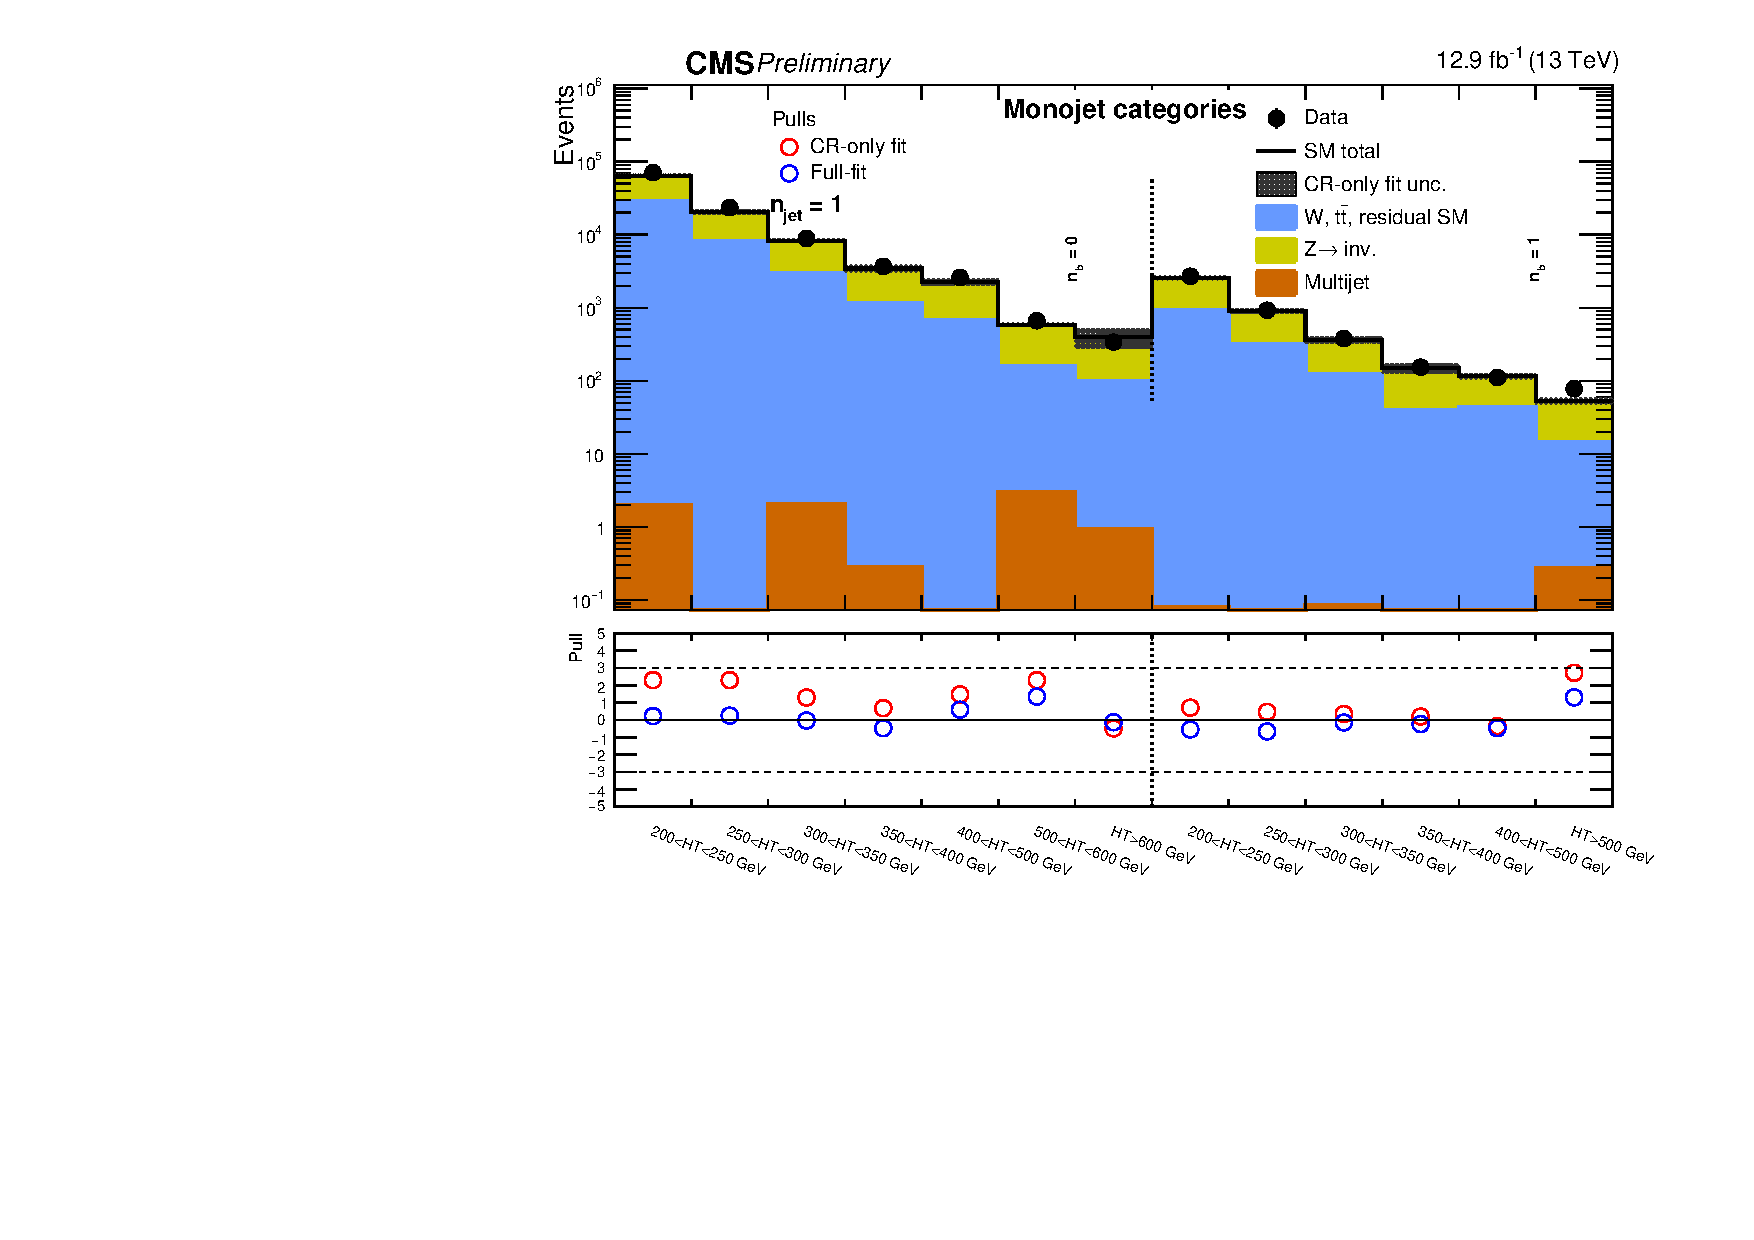
\includegraphics[width=0.7\textwidth]{summaryPlot_Monojet_prefit_overlay_fit_b}
    \caption{(Top panel) Event yields observed in data (solid circles)
      and SM expectations with their associated uncertainties (black
      histogram with shaded band) from a CR-only fit as a function of
      \nb and \scalht for the monojet topology ($\njet = 1$) in the
      signal region. (Bottom panel). The significance of deviations
      (pulls) observed in data with respect to the SM expectations
      from the CR-only (red circles) and full fit (blue circles). The
      pulls are indicative only and cannot be considered
      independently.}
    \label{fig:mono}
  \end{center}
\end{figure}

\begin{figure*}[!h]
  \begin{center}
    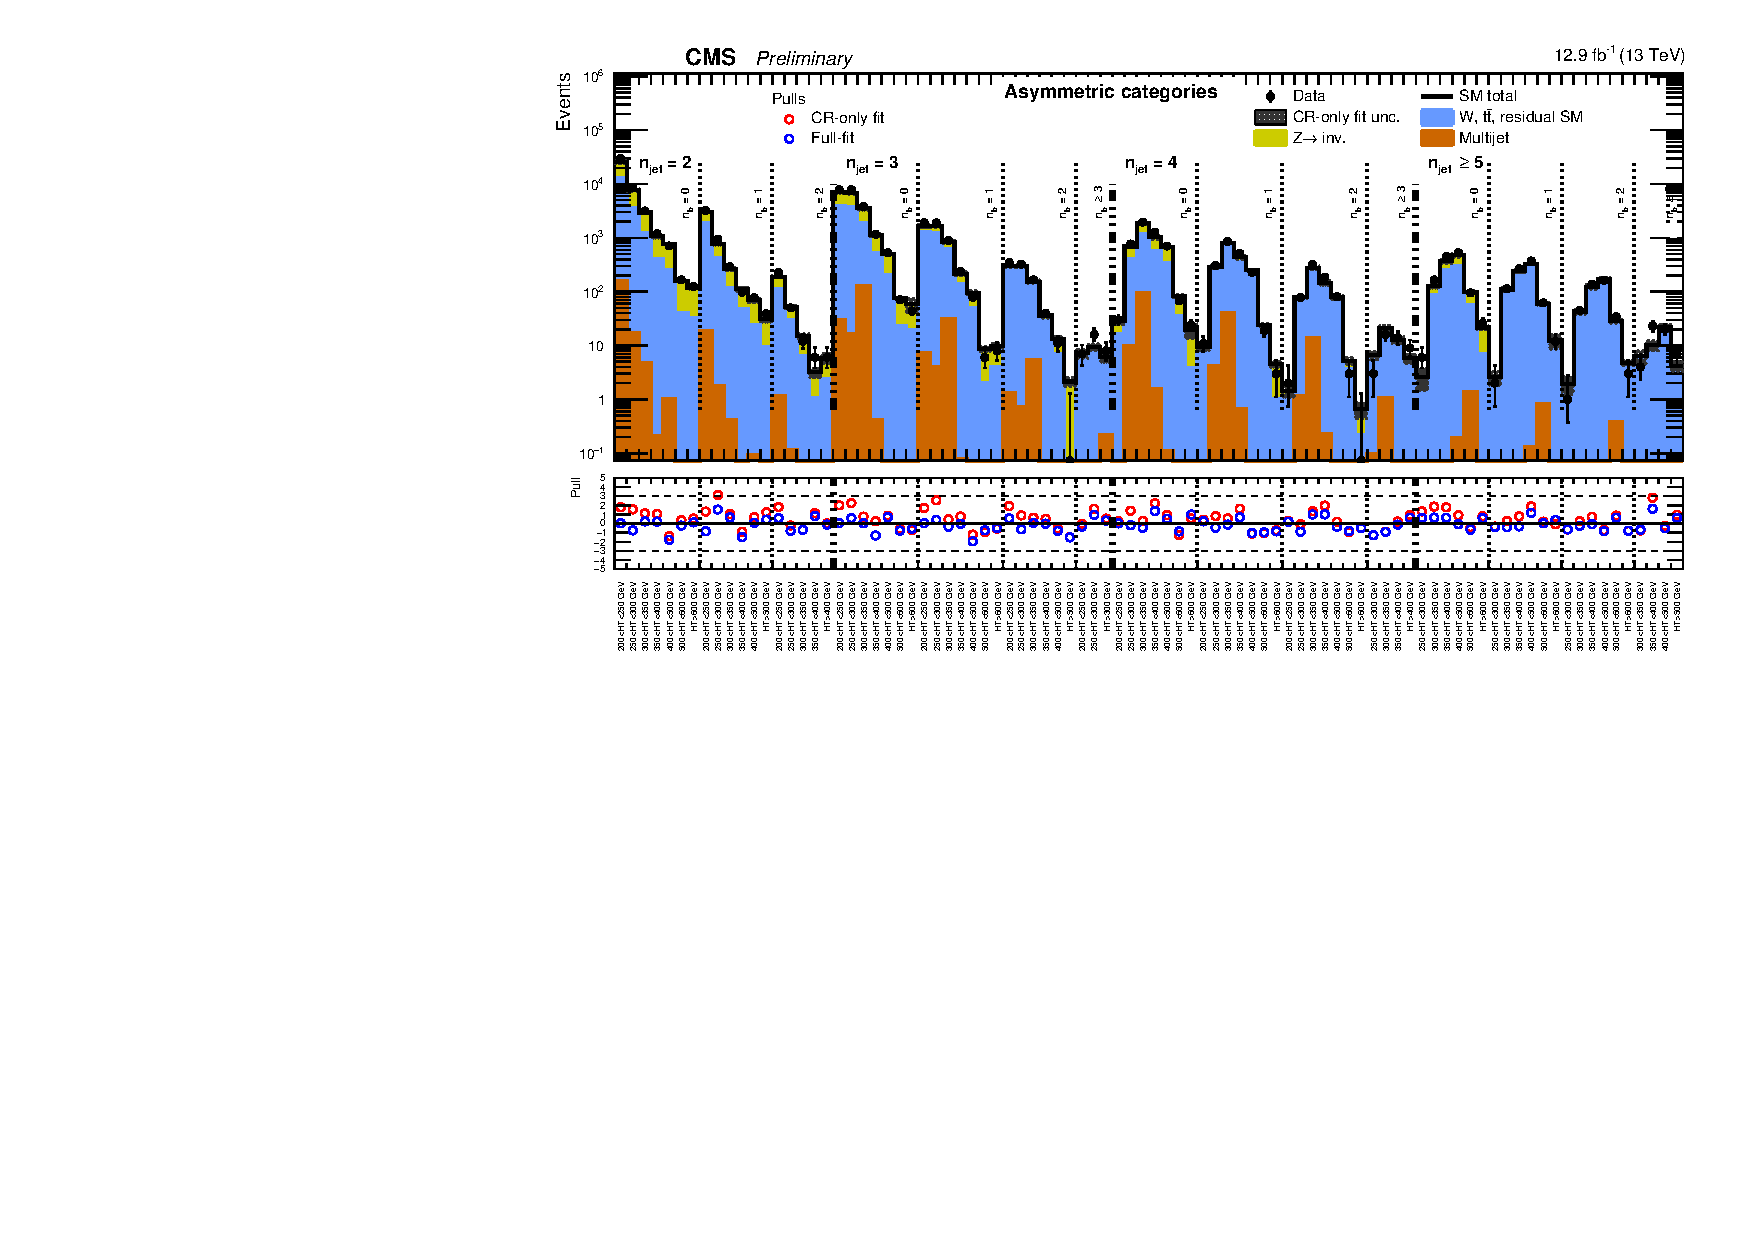
\includegraphics[angle=90,width=0.7\textwidth]{summaryPlot_Asymmetric_prefit_overlay_fit_b}
    \caption{(Top panel) Event yields observed in data (solid circles)
      and SM expectations with their associated uncertainties (black
      histogram with shaded band) from a CR-only fit, integrated over
      \HTmiss, as a function of \njet, \nb, and \scalht for the
      asymmetric topology in the signal region. (Bottom panel). The
      significance of deviations (pulls) observed in data with respect
      to the SM expectations from the CR-only (red circles) and full
      fit (blue circles). The pulls are indicative only and cannot be
      considered independently.}
    \label{fig:asym}
  \end{center}
\end{figure*}

\begin{figure*}[!h]
  \begin{center}
    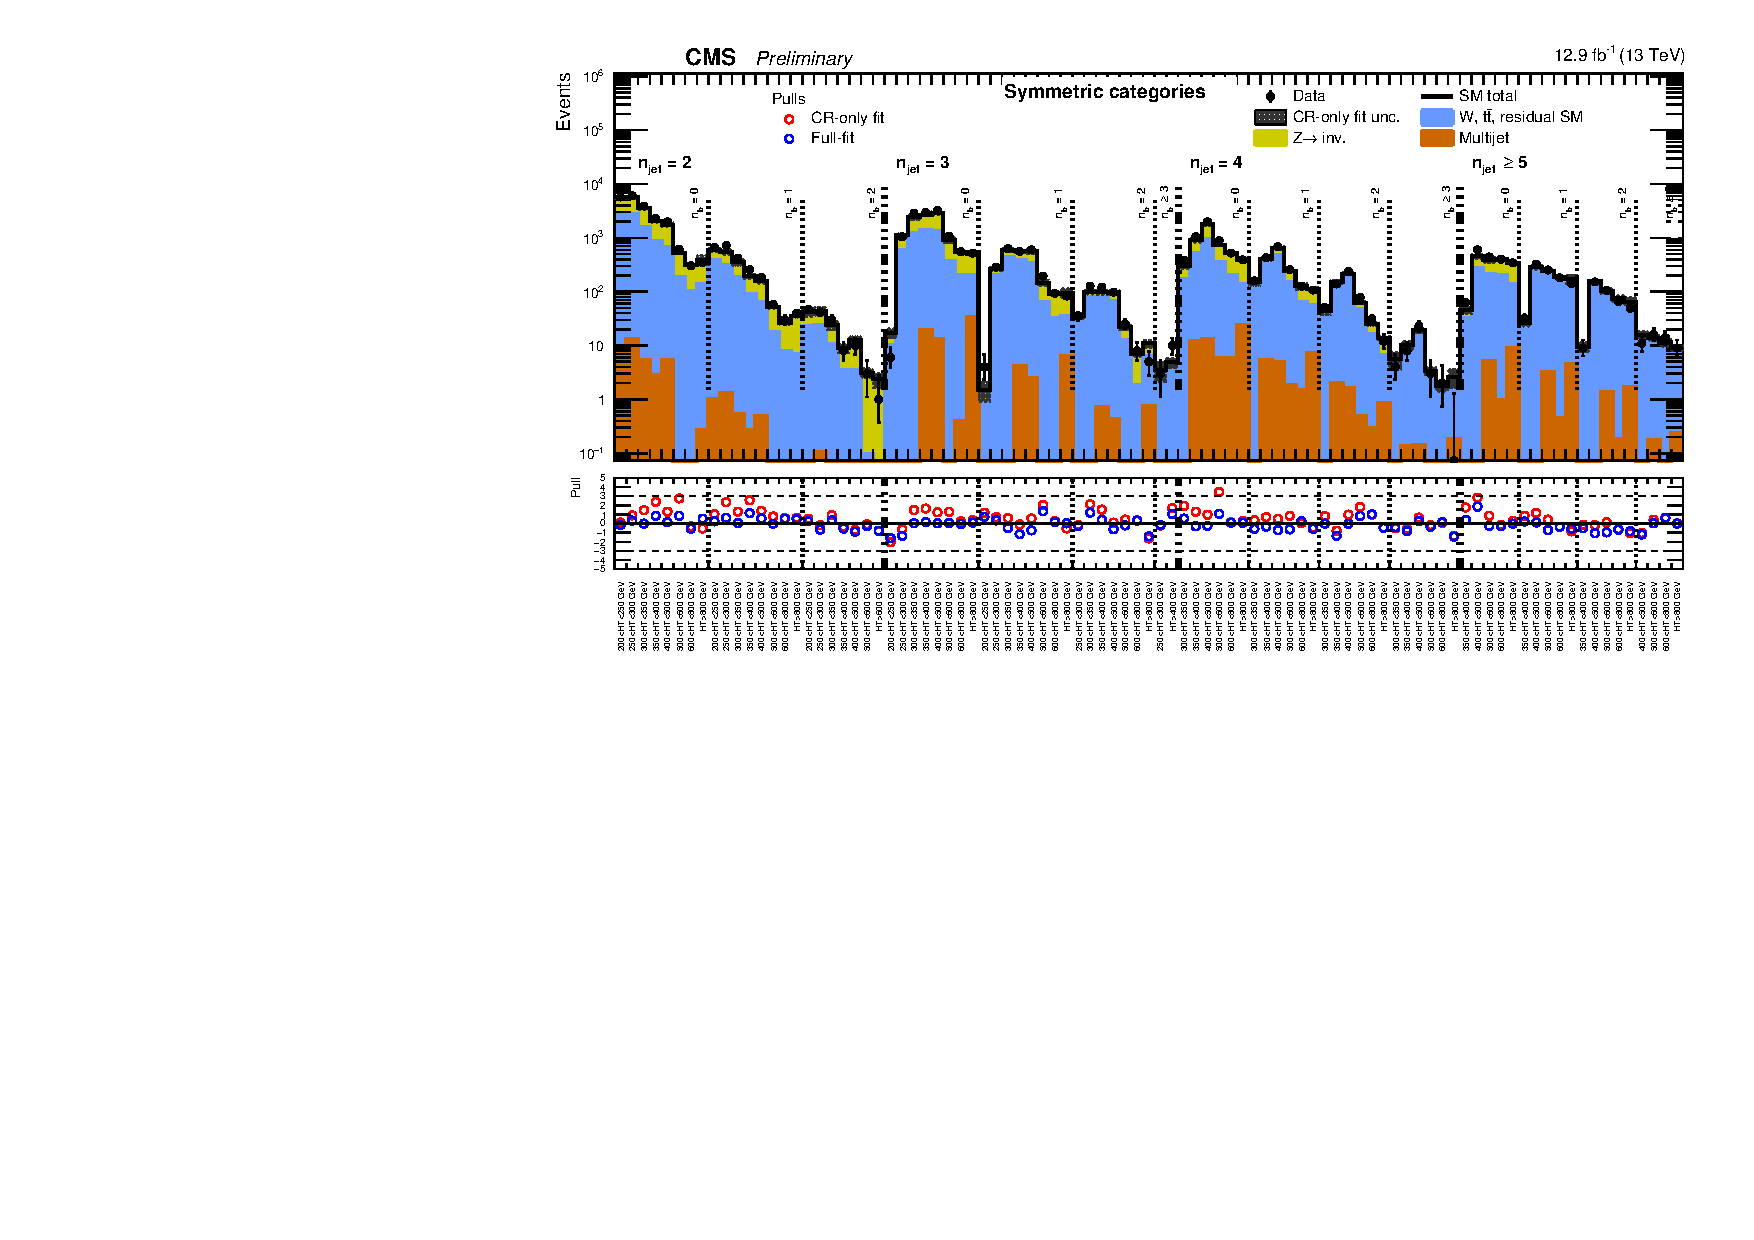
\includegraphics[angle=90,width=0.7\textwidth]{summaryPlot_Symmetric_prefit_overlay_fit_b}
    \caption{(Top panel) Event yields observed in data (solid circles)
      and SM expectations with their associated uncertainties (black
      histogram with shaded band) from a CR-only fit, integrated over
      \HTmiss, as a function of \njet, \nb, and \scalht for the
      symmetric topology in the signal region. (Bottom panel). The
      significance of deviations (pulls) observed in data with respect
      to the SM expectations from the CR-only (red circles) and full
      fit (blue circles). The pulls are indicative only and cannot be
      considered independently.}
    \label{fig:sym}
  \end{center}
\end{figure*}


%%__________________________________________________________________||
